\section{Radiation Transport}
\label{sec:bg:rt}

Radiation transport is good content.

\subsection{Transport Equation}

\begin{multline}\label{bg:eq:transport}
  \hat{\Omega}\cdot\vec{\nabla}\psi\left(\vec{r},\hat{\Omega},E\right) +
  \sigma_t\left(\vec{r},E\right)\psi\left(\vec{r},\hat{\Omega},E\right) - \\
  \iint\sigma_s\left(\vec{r},\hat{\Omega}^\prime\rightarrow\hat{\Omega},E^\prime\rightarrow E\right)\psi\left(\vec{r},\hat{\Omega}^\prime,E^\prime\right)d\hat{\Omega}^\prime dE^\prime =
  q\left(\vec{r},\hat{\Omega},E\right)
\end{multline}

The transport equation is defined by Equation \ref{bg:eq:transport}.

\subsection{Monte Carlo Radiation Transport}
\label{sec:bg:mc}

Reference to \ac{mcnp} \cite{mcnp5-theory}.

As described in Section \ref{sec:bg:rt}, radiation transport is good content.
But Monte Carlo radiation transport is even better content.

Figure \ref{fig:bg:flux} shows an example figure.

\begin{figure}[h!]
  \centering
  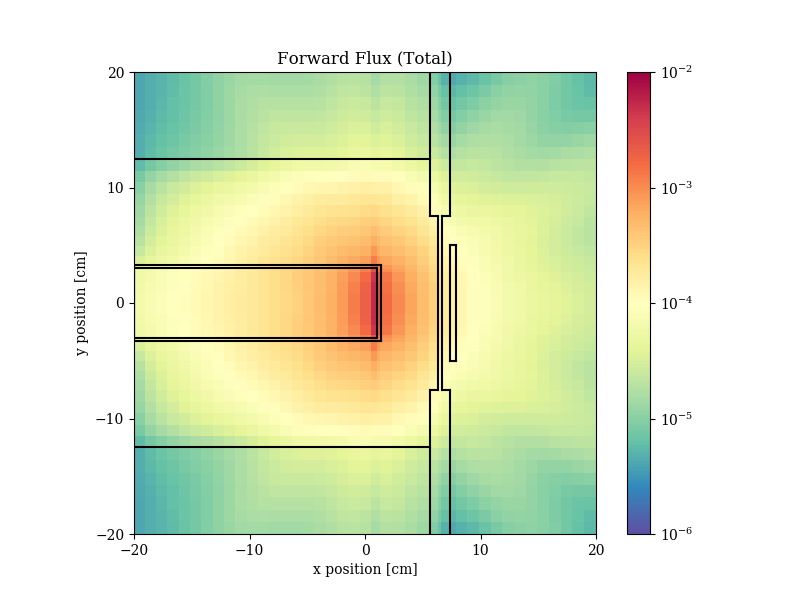
\includegraphics[width=1.0\textwidth]{content/scalar_flux_fwd_total.png}
  \caption[Short figure caption]{Long figure caption}
  \label{fig:bg:flux}
\end{figure}

Table \ref{tab:bg:mats} shows an example table.

\begin{table}[h]
  \centering
  \caption[Short table caption]{Long table caption}
  \label{tab:bg:mats}
  \begin{tabular}{| c | c | c |}
    \hline
    \textbf{Material ID} & \textbf{Material} \\ \hline
     0 & Void                 \\ \hline
     1 & Air                  \\ \hline
     2 & Aluminum             \\ \hline
     3 & Beryllium            \\ \hline
     4 & Beryllium oxide      \\ \hline
     5 & Boron                \\ \hline
     6 & Graphite             \\ \hline
     7 & Copper               \\ \hline
     8 & Iron                 \\ \hline
     9 & Borated polyethylene \\ \hline
    10 & Polyethylene         \\ \hline
    11 & Heavy water          \\ \hline
    12 & Light water          \\ \hline
    13 & Uranium-235          \\ \hline
  \end{tabular}
\end{table}
